% !TeX root = bash.tex
\section{III. Pipes}
\begin{frame}
\frametitle{stdout}
When you \tt{printf}, where does the string go?
\newline \newline
Your screen? Yes but also no.
\newline \newline
\tt{stdout}, or \textbf{standard output}, is a special file where \tt{printf}
dumps its output.\footnote{Yes, there's \tt{stderr} too, but we won't be talking
about it.}
\end{frame}

\begin{frame}[fragile]
\frametitle{Capturing stdout}
You can capture the stdout of a command and direct it somewhere else than your
screen, such as a file.
Try this:
\begin{lstlisting}[language=bash]
$ echo hello        # print to terminal
$ echo hello > out  # write to file
\end{lstlisting}
\begin{figure}
    \centering
    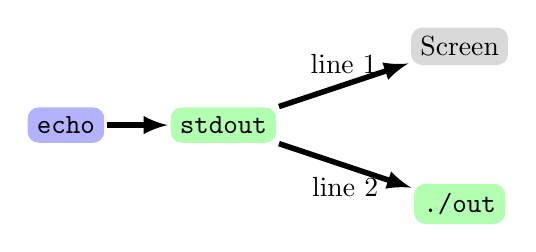
\begin{tikzpicture}
        \tikzstyle{every node}=[rounded corners]
        \node[fill=blue!30]  (prog)        at (0,  0) {\tt{echo}};
        \node[fill=green!30] (stdout)      at (2,  0) {\tt{stdout}};
        \node[fill=gray!30]  (term)        at (5,  1) {Screen};
        \node[fill=green!30] (stdout-file) at (5, -1) {\tt{./out}};
        \tikzstyle{every node}=[fill=none]
        \draw[-latex] (prog) -- (stdout);
        \draw[-latex] (stdout) -- (term) node[above,midway] {line 1};
        \draw[-latex] (stdout) -- (stdout-file) node[below,midway] {line 2};
    \end{tikzpicture}
\end{figure}
\end{frame}

\begin{frame}[fragile]
\frametitle{\tt{>} and \tt{>>}}
Try \tt{>>} instead of \tt{>}. What happens?
\begin{lstlisting}[language=bash]
$ echo hello >> out
$ cat out
\end{lstlisting}
Repeat a few times with both \tt{>} and \tt{>>}. What's the difference?
\pause
\begin{block}{Observation}
    \tt{>} overwrites the file, but \tt{>>} appends to it.
\end{block}
\end{frame}

\begin{frame}[fragile]
\frametitle{stdin}
The opposite of \tt{stdout} is \tt{stdin}: standard input.
Some programs read from stdin when they expect a path but aren't given any.
\newline \newline
Try this in \tt{03-pipes/}:
\begin{lstlisting}[language=bash]
$ ls random/ | head -n 5
\end{lstlisting}
\pause
\begin{block}{Observation}
    Normally \tt{head} expects a filename, but when none is given, it
    falls back to stdin — which is what \tt{ls} printed to stdout.
\end{block}
\begin{block}{Convention}
    We sometimes call the vertical bar (\tt{|}) the \textbf{pipe} character.
\end{block}
\end{frame}

\begin{frame}[fragile]
\frametitle{The power of pipes}
You can chain commands with pipes. Classic recipe (still in \tt{03-pipes}):
\begin{lstlisting}[language=bash]
$ cat numbers
$ cat numbers | sort
$ cat numbers | sort | uniq
$ cat numbers | sort | uniq | wc
\end{lstlisting}
\pause
\begin{block}{Observations}
    \begin{itemize}
        \item Each program takes the last one's stdout as stdin
        \item Only the final program will print to terminal
    \end{itemize}
\end{block}
\begin{block}{Explanation}
    \begin{itemize}
        \item By default, \tt{sort} sorts stdin in dictionary order
            (check man page for more)
        \item \tt{wc} is short for ``word count'', although the first thing
            it prints is the number of lines.
    \end{itemize}
\end{block}
\end{frame}

\begin{frame}[fragile]
\frametitle{Pipes illustrated}
\begin{lstlisting}[language=bash]
$ cat numbers | sort | uniq | wc
\end{lstlisting}
\begin{figure}
    \centering
    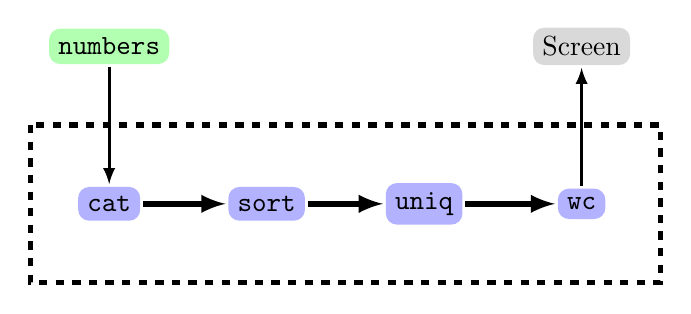
\begin{tikzpicture}
        \tikzstyle{every node}=[fill=blue!30, rounded corners]
        \node[fill=green!30] (numbers) at (-2, 2) {\tt{numbers}};
        \node (cat)         at (-2, 0) {\tt{cat}};
        \node (sort)        at (0,  0) {\tt{sort}};
        \node (uniq)        at (2,  0) {\tt{uniq}};
        \node (wc)          at (4,  0) {\tt{wc}};
        \node[fill=gray!30] (term) at (4,  2) {Screen};
        \tikzstyle{every node}=[fill=none]
        \tikzstyle{every path}=[-latex,line width=2pt]
        \draw[line width=1pt] (numbers) -- (cat);
        \draw (cat) -- (sort);
        \draw (sort) -- (uniq);
        \draw (uniq) -- (wc);
        \draw[line width=1pt] (wc) -- (term);
        \draw[dashed] (-3, 1) rectangle (5, -1);
    \end{tikzpicture}
\end{figure}
\begin{block}{Challenge}
    Can you think of a way to eliminate a pipe? (Hint: man sort)
    % sort numbers | uniq | wc
\end{block}
\end{frame}

\begin{frame}[fragile]
\frametitle{grep}
Try this in \tt{03-pipes}:
\begin{lstlisting}[language=bash]
$ ls random/ | grep JI
\end{lstlisting}
\pause
\begin{block}{Explanation}
    \tt{grep} is a powerful tool to match a substring. By default, it takes
    a file (or stdin), and prints all lines containing a pattern (``JI'').
\end{block}
\end{frame}

\begin{frame}
\frametitle{Challenge}
Inside \tt{03-pipes/random/}:
\begin{itemize}
    \item List all filenames containing ``FDU''
    \item List all filenames containing ``UM'' (upper and lower cases)
        (Hint: man grep)
    \item List all filenames containing ``UM'' but not ``FDU''
        (upper and lower cases for both substrings)
\end{itemize}
\end{frame}

\begin{frame}[fragile]
\frametitle{Solution}
\begin{lstlisting}[language=bash]
$ ls | grep FDU
$ ls | grep -i UM
$ ls | grep -i UM | grep -i -v FDU
\end{lstlisting}
\end{frame}

\begin{frame}
\frametitle{Conclusion}
\begin{itemize}
    \item Files and directories form a tree
    \item One tool does one thing, but flags specify how
    \item When in doubt, read documentation
    \item Chain together tools and unleash immense power
\end{itemize}
\end{frame}
